\documentclass[RNAAS]{aastex631}

\usepackage{amsmath}

\shorttitle{PowerSpectR}
\shortauthors{de Souza}
\graphicspath{{./}{figures/}}

\begin{document}

\title{PowerSpectR: Robust Median-Based Power Spectrum Analysis for Astronomical Images}

\correspondingauthor{Rafael S. de Souza}
\email{rd23aag@herts.ac.uk}

\author[0000-0001-7207-4584]{Rafael S. de Souza}
\affiliation{Centre for Astrophysics Research, University of Hertfordshire, College Lane, Hatfield, AL10 9AB, UK}
\affiliation{Instituto de Fisica, Universidade Federal do Rio Grande do Sul, Porto Alegre, RS 90040-060, Brazil}
\affiliation{Department of Physics \& Astronomy, University of North Carolina at Chapel Hill, NC 27599-3255, USA}

\begin{abstract}
We introduce \texttt{PowerSpectR}, an \textsf{R} package for computing and visualizing robust, median-based Fourier power spectra from two-dimensional astronomical images. The package provides a compact workflow for estimating the slope of scale-free spatial structure by combining azimuthal median statistics with radial binning in Fourier space. This medianized estimator is less sensitive than mean-based alternatives to bright compact sources, residual artifacts, and incomplete masks. \texttt{PowerSpectR} is implemented in \textsf{R} and released under the MIT license at \url{https://github.com/RafaelSdeSouza/PowerSpectR}.
\end{abstract}

\keywords{Astrostatistics (1882) --- Astronomical software (1855) --- Fourier analysis (1967)}

\section{Motivation}

Two-dimensional power spectra are widely used to quantify the spatial structure of astronomical images, where the fitted slope encodes how power is distributed across scales. In many practical applications, however, the usual azimuthal \emph{mean} of the squared Fourier amplitudes is fragile: a few bright stars, cosmic rays, deblending residuals, or masked regions can bias the inferred spectrum. Median-based estimators offer a more stable alternative while preserving the scale dependence of the signal. Motivated by their use in turbulence and structure analysis \citep[e.g.,][]{Burkhart2013}, we developed \texttt{PowerSpectR} as a lightweight, reproducible \textsf{R} package for robust radial power-spectrum estimation.

\section{Methodology}

Given an image \(I(x, y)\) with dimensions \(h \times w\), the package first subtracts the image mean and applies a two-dimensional Hann window \(W(x, y)\) to suppress edge effects. The power spectrum is then
\begin{equation}
P(k_x, k_y) = \left| \mathcal{F}\left\{ W(x,y)\,[I(x,y) - \bar{I}] \right\} \right|^2,
\end{equation}
where \(\mathcal{F}\{\cdot\}\) denotes the discrete Fourier transform. After FFT shifting, the radial coordinate
\begin{equation}
k = \sqrt{k_x^2 + k_y^2}
\end{equation}
is binned and summarized with the azimuthal median,
\begin{equation}
\tilde{P}(k_j) = \mathrm{median}\!\left\{ P(k_x, k_y)\,:\, k \in [k_j^{\mathrm{min}}, k_j^{\mathrm{max}}] \right\}.
\end{equation}
The fitted spectral slope \(\beta\) is obtained from a linear model in log--log space,
\begin{equation}
\log \tilde{P}(k) = \alpha + \beta \log k + \varepsilon,
\end{equation}
where \(\varepsilon\) captures stochastic fluctuations around the trend.

\section{Example}

The user-facing interface is centered on \texttt{global\_psd()}, which performs the windowing, Fourier transform, radial medianization, and slope fitting, and \texttt{plot\_power\_spectrum()}, which produces a quick diagnostic plot. A minimal workflow is
\begin{verbatim}
res <- global_psd("m101_hubble.jpg", nbins = 60,
                  drop_bins = 2, window = "hann")
plot_power_spectrum(res)
\end{verbatim}

Figure~\ref{fig:hubble-comparison} illustrates the workflow on a matched pair of Hubble Space Telescope cutouts. The spiral galaxy M101 retains more small-scale power and yields a flatter fitted slope (\(\beta \approx -1.78\)) than the smoother elliptical galaxy M60 (\(\beta \approx -2.36\)). This example highlights how the package can distinguish morphologically structured and centrally concentrated light distributions using the same analysis pipeline.

\begin{figure}[t]
\centering
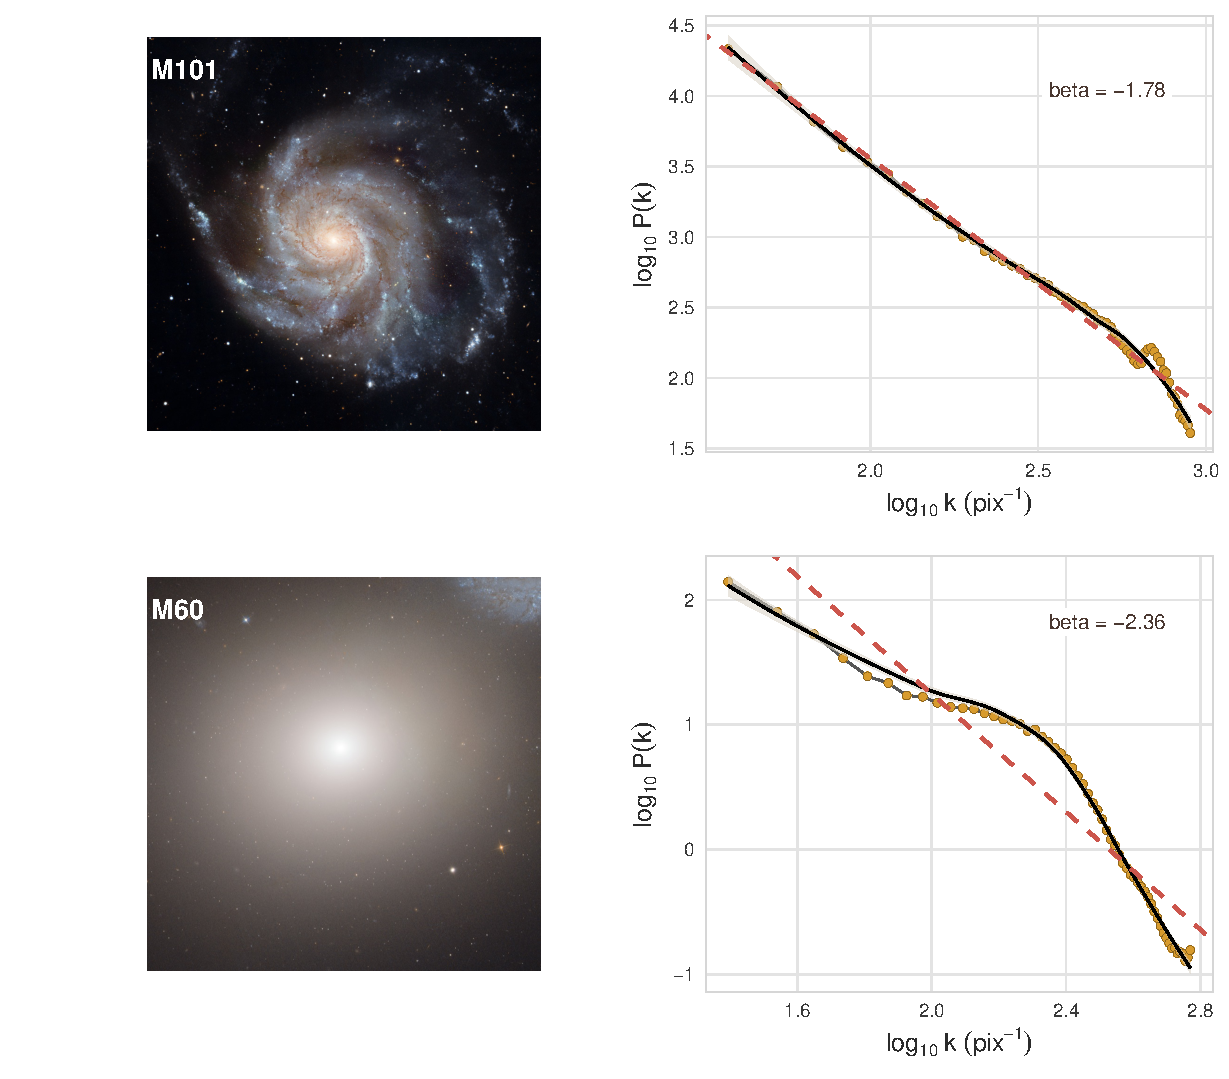
\includegraphics[width=\linewidth]{hubble_morphology_mosaic.pdf}
\caption{Matched-telescope comparison using cropped public Hubble color images of the spiral galaxy M101 and the elliptical galaxy M60. The left column shows the galaxy cutouts and the right column shows their corresponding median radial power spectra estimated by \texttt{PowerSpectR}. The fitted slopes are \(\beta \approx -1.78\) for M101 and \(\beta \approx -2.36\) for M60. The image cutouts were adapted from the NASA Science assets ``Hubble Image of M101'' and ``Elliptical Galaxy M60'' \citep{NASAM101Image,NASAM60Image}.\label{fig:hubble-comparison}}
\end{figure}

\section{Applications and Extensions}

Although developed with astronomical imaging in mind, the same workflow applies to emission-line maps, narrow-band slices from integral-field spectroscopy, dust-column maps, and remote-sensing textures. Planned extensions include explicit masked-pixel handling, broken power-law fits, and multiscale wavelet diagnostics that complement the global spectral slope.

\begin{acknowledgments}
R.S.S. acknowledges support from the Conselho Nacional de Desenvolvimento Cientifico e Tecnologico (CNPq, Brazil, grants 446508/2024-1 and 315026/2025-1). The author thanks the open-source \textsf{R} community for the tools that made this package possible.
\end{acknowledgments}

\software{R \citep{RCoreTeam2025}, imager \citep{Barthelme2025}, ggplot2 \citep{Wickham2016}, cowplot \citep{Wilke2025}}

\bibliography{ref}{}
\bibliographystyle{aasjournal}

\end{document}
